\section{User Study: Restocking}
\label{sec:user_study}
All experiments so far used author-collected demonstrations. Because an LfD method's performance depends on the user, we conduct a study with 10 participants of varying familiarity with kinesthetic teaching and LfD, on a restocking task adapted from Ajanovi\'c et al.~\cite{11369949}. Their supermarket scenario used fixed object locations; our adaptation tracks the bottle and basket dynamically, so the localizer must generalize across spatial configurations. They found that users' preferences varied widely and that segmented demonstrations yielded slightly smoother, more successful policies at the cost of more demonstration time, supporting our use of segmented demonstrations.

\begin{figure*}[t]
\centering
% Photo crops of the old restocking_banner.png (Figures/exp_frames/rst_*.png);
% replace with high-res originals (same filenames) when available.
\resizebox{\textwidth}{!}{%
\begin{tikzpicture}[font=\small,
  photo/.style={inner sep=0pt}, lbl/.style={font=\scriptsize, align=center}]
\node[photo] (r1) {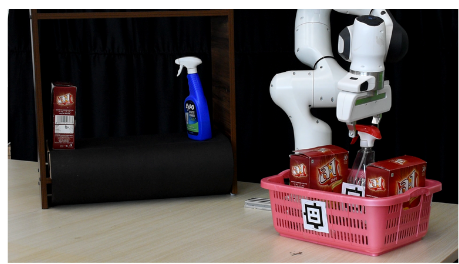
\includegraphics[height=2.9cm]{Figures/exp_frames/rst_grasptop.png}};
\node[photo, right=2mm of r1] (r2) {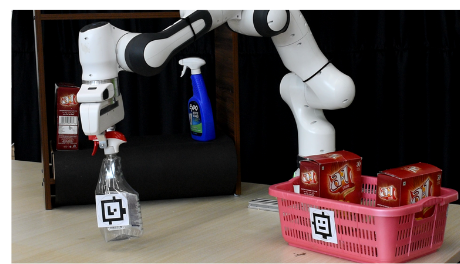
\includegraphics[height=2.9cm]{Figures/exp_frames/rst_placetable.png}};
\node[photo, right=2mm of r2] (r3) {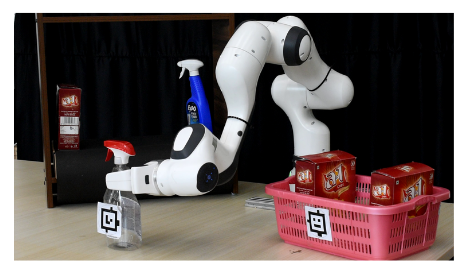
\includegraphics[height=2.9cm]{Figures/exp_frames/rst_graspside.png}};
\node[photo, right=2mm of r3] (r4) {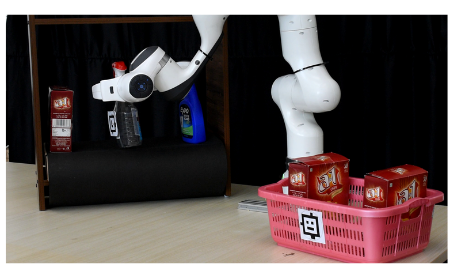
\includegraphics[height=2.9cm]{Figures/exp_frames/rst_placeshelf.png}};
\node[lbl, below=1mm of r1] {1.\ \textit{Grasp\_Top}};
\node[lbl, below=1mm of r2] {2.\ \textit{Place\_Table}};
\node[lbl, below=1mm of r3] {3.\ \textit{Grasp\_Side}};
\node[lbl, below=1mm of r4] {4.\ \textit{Place\_Shelf}};
\draw[->, thick] (r1) -- (r2); \draw[->, thick] (r2) -- (r3); \draw[->, thick] (r3) -- (r4);
\end{tikzpicture}%
}

\caption{\textbf{Restocking task.} The nominal sequence \textit{Grasp\_Top} $\to$ \textit{Place\_Table} $\to$ \textit{Grasp\_Side} $\to$ \textit{Place\_Shelf}: a cluttered basket forces the top grasp and the low shelf forces the side grasp, so the decomposition isolates the effect of SEAL's active-learning loop.}
\label{fig:restocking_banner}
\end{figure*}

Because a cluttered basket forces a top grasp and a low shelf forces a side grasp, the task decomposes into \textit{Grasp\_Top}, \textit{Place\_Table}, \textit{Grasp\_Side}, \textit{Place\_Shelf} (Fig.~\ref{fig:restocking_banner}). We fix the features via the LLM so that only demonstration quality and diversity vary. The protocol: (1) participants give two segmented demonstrations aiming to maximize diversity (the \emph{Unguided} baseline); (2) we seed the GPC with the first demonstration and select 4 uncertain points (two gripper-open, two gripper-closed) via center-weighted epistemic uncertainty; (3) for each point we set up the corresponding scene and ask the participant to label and demonstrate the correct action to completion, yielding 4 sub-demonstrations that, with the first demonstration, form the \emph{SEAL Guided} set; (4) participants answer qualitative questions after each condition. We keep the count at 2 to probe the low-data regime and because participant frustration rose with more demonstrations; requesting 4 short sub-demonstrations (rather than 4 full ones) keeps the SEAL set comparable in points and collection time to the Unguided set while being more intuitive.

We test three hypotheses: (H1) even when explicitly asked to maximize diversity, users produce demonstrations with large state-space overlap; (H2) demonstrations elicited at SEAL's uncertainty queries yield a better classifier than the same user's unguided demonstrations; (H3) users prefer the SEAL protocol. The final dataset comprises 20 sets (one Unguided, one SEAL per participant).

{\color{magenta}\textbf{Diversity (H1).} Since the first demonstration is shared, we measure the Directed Chamfer Distance (DCD) from points in subsequent demonstrations to same-mode points in the first,
$$\text{DCD}(A,B)=\frac{1}{|B|}\sum_{b\in B}\min_{a\in A}\|a-b\|.$$
The SEAL set ($\mu{=}0.247,\sigma{=}0.078$) is significantly more diverse than the Unguided baseline ($\mu{=}0.096,\sigma{=}0.108$; Wilcoxon $W=2.0, p=0.0059$, effect size $r=0.927$). To contextualize these unitless scalar values, we evaluate them relative to the maximum geometric scale of the feature space. Because the spatial and angular axes are normalized to a unit square, the theoretical bounding box diagonal is strictly $\sqrt{2}$. The Unguided figure provides direct evidence for H1: despite explicit instructions to maximize diversity, participants' second demonstrations stayed on average within just $6.8\%$ of the total feature range of their first. In contrast, SEAL successfully forced users to deviate, driving exploration across $17.5\%$ of the global feature space.} \todo{MMD anchor (co-author): 0.096 is unitless to the reader. Compute a reference scale from the study data---e.g., the diagonal of the $F_{\min}$ bounding box over all demonstrations, or the mean pairwise distance between points of DIFFERENT modes---and restate both MMDs as percentages of it (``Unguided demonstrations stayed within $\sim$X\% of the feature range of the first demonstration''). One line of numpy on the logged study data.}  \todo{given $N{=}10$, add Wilcoxon signed-rank and an effect size alongside each $t$-test in this section (H1 MMD, H2 paired mIoU, H3 mental effort)} \textbf{STATUS: DONE} Because classifier accuracy is a property of the data rather than of who staged the scene, this and the mIoU result below are robust to the scene-setup confound noted in Sec.~\ref{sec:limitations}.

\textbf{Classifier performance (H2).} We train 10 GPCs per dataset and report mIoU against a ground-truth classification defined by an independently hand-designed automaton over the full feature set (not from any trained model, hence non-circular). {\color{magenta} To control for individual expertise and account for repeated measures, we aggregated trial scores to evaluate the mean performance per participant. Overall, SEAL significantly improved  mIoU ($0.817 \pm 0.079$ vs $0.728 \pm 0.107$; $W=7.0, p=0.037$, effect size $r=0.745$). Focusing on the per-participant \emph{relative} change (Fig.~\ref{fig:participant_perf}), 7 of 10 participants improved with SEAL and 2 others changed within training-run variance, supporting H2. One participant (P09) declined markedly: they provided labels inconsistent with the ground-truth classification during the SEAL sub-demonstrations, underscoring the method's dependence on label quality (Sec.~\ref{sec:limitations}).} (\todo{report the paired test over the 10 per-participant mIoU pairs---Wilcoxon signed-rank $W$, $p$, effect size}) \textbf{STATUS:DONE}


\begin{figure}[htbp]
\centering
% Redrawn in pgfplots from the value labels of the old pref.png.
\begin{tikzpicture}
\begin{axis}[
  ybar, 
  bar width=12pt, % Increased bar width
  width=0.85\columnwidth, % Reduced overall width to shrink space between groups
  height=5.2cm,
  ymin=0, ymax=10.5, % Slightly increased ymax to give the top labels breathing room
  ylabel={\# participants},
  symbolic x coords={SEAL,Unguided,Both}, xtick=data,
  enlarge x limits=0.25, % Tightened outer margins slightly
  legend style={at={(0.97,0.97)}, anchor=north east, font=\scriptsize},
  nodes near coords, 
  every node near coord/.append style={
      font=\scriptsize\bfseries % Added bold to match previous style, but kept position default (above bars)
  },
  tick label style={font=\scriptsize}, label style={font=\scriptsize},
]
\addplot[fill=seal!25, draw=seal!60]      coordinates {(SEAL,6) (Unguided,4) (Both,0)};
\addplot[fill=seal!60, draw=seal]         coordinates {(SEAL,7) (Unguided,2) (Both,0)};
\addplot[fill=seal, draw=seal!50!black]   coordinates {(SEAL,6) (Unguided,4) (Both,0)};
\legend{usage comfort, trust, perceived effectiveness}
\end{axis}
\end{tikzpicture}
\caption{\textbf{User preferences:} more users prefer SEAL guidance over Unguided demonstrations on Comfort, Trust, and Perceived Effectiveness in a head-to-head comparison ($N{=}10$; no participant chose ``Both'').}
\label{fig:user_pref}

\vspace{2em} % Controls the exact spacing between the two plots

\pgfplotsset{compat=1.18}
\definecolor{ugpink}{RGB}{242, 165, 172}
\definecolor{slgreen}{RGB}{168, 211, 183}

% Redrawn in pgfplots to match "miou.png"
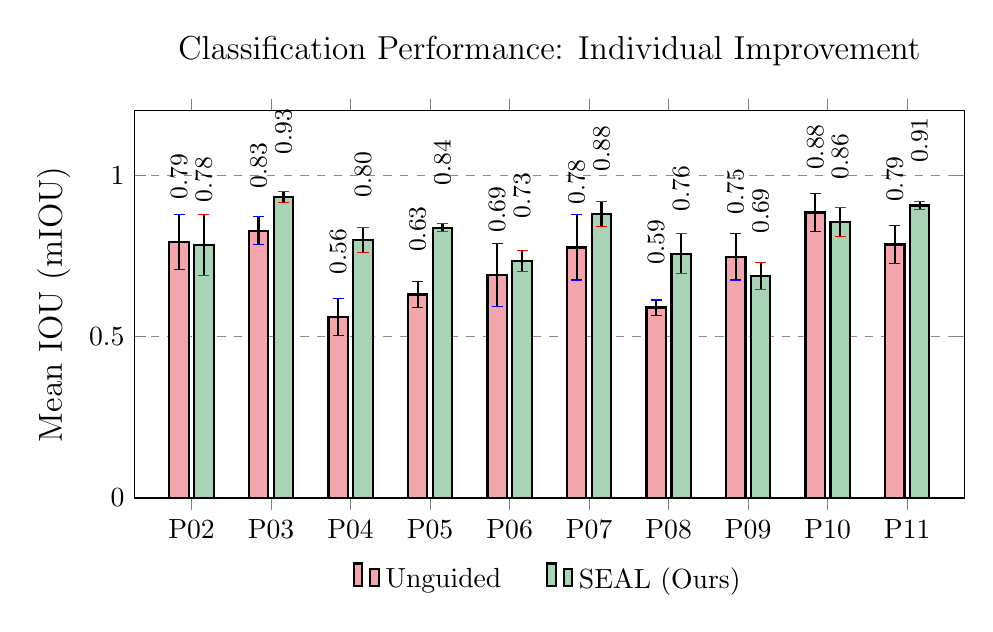
\begin{tikzpicture}
\begin{axis}[
  width=\columnwidth, % Made the plot wider
  height=6.5cm,
  ybar, bar width=7pt, % Made the bars thinner
  ymin=0, ymax=1.2, % Increased ymax to accommodate text above bars
  ylabel={Mean IOU (mIOU)},
  title={Classification Performance: Individual Improvement},
  title style={font=\large, yshift=1.5ex},
  symbolic x coords={P02,P03,P04,P05,P06,P07,P08,P09,P10,P11},
  xtick=data,
  enlarge x limits=0.08,
  ymajorgrids=true, 
  grid style={dashed, darkgray!60},
  legend style={
      at={(0.5,-0.15)}, 
      anchor=north, 
      legend columns=2, 
      draw=none, 
      font=\normalsize,
      /tikz/every even column/.append style={column sep=0.5cm}
  },
  nodes near coords,
  point meta=explicit symbolic,
  every node near coord/.append style={
      font=\small,
      rotate=90,
      anchor=west, % Anchors the text ABOVE the bar
      text=black,
      inner xsep=15pt, % Adds tolerance (spacing) above the bar
      yshift=0pt % Shifts text slightly right to avoid clashing directly with the error bar
  },
  tick label style={font=\normalsize}, 
  label style={font=\large},
]

% Unguided
\addplot+[
    fill=ugpink, draw=black, thick,
    error bars/.cd, y dir=both, y explicit,
    error bar style={thick}
] coordinates {
    (P02,0.7923) +- (0,0.0857) [0.79]
    (P03,0.8278) +- (0,0.0438) [0.83]
    (P04,0.5609) +- (0,0.0571) [0.56]
    (P05,0.6305) +- (0,0.0396) [0.63]
    (P06,0.6903) +- (0,0.0983) [0.69]
    (P07,0.7763) +- (0,0.1010) [0.78]
    (P08,0.5899) +- (0,0.0236) [0.59]
    (P09,0.7468) +- (0,0.0716) [0.75]
    (P10,0.8844) +- (0,0.0585) [0.88]
    (P11,0.7854) +- (0,0.0595) [0.79]
};

% SEAL (Ours)
\addplot+[
    fill=slgreen, draw=black, thick,
    error bars/.cd, y dir=both, y explicit,
    error bar style={thick}
] coordinates {
    (P02,0.7837) +- (0,0.0941) [0.78]
    (P03,0.9328) +- (0,0.0170) [0.93]
    (P04,0.7999) +- (0,0.0391) [0.80]
    (P05,0.8370) +- (0,0.0126) [0.84]
    (P06,0.7342) +- (0,0.0318) [0.73]
    (P07,0.8807) +- (0,0.0387) [0.88]
    (P08,0.7567) +- (0,0.0618) [0.76]
    (P09,0.6866) +- (0,0.0417) [0.69]
    (P10,0.8558) +- (0,0.0448) [0.86]
    (P11,0.9061) +- (0,0.0136) [0.91]
};

\legend{Unguided, SEAL (Ours)}
\end{axis}
\end{tikzpicture}
\caption{\textbf{mIoU per participant} for SEAL- and Unguided-trained models, averaged over 10 runs; error bars show $\pm1$ SD.}
\label{fig:participant_perf}
\end{figure}

\textbf{Preferences (H3).} More participants preferred SEAL on Ease of Use, Trust, and Efficiency (Fig.~\ref{fig:user_pref}), though these majorities did not reach statistical significance (Binomial $p > 0.05$). Self-reported mental effort dropped with SEAL ($2.6\!\to\!1.8$, $p=0.125$), but physical-effort and ``how hard to achieve a good demonstration'' items showed no significant difference. H3 is thus only partially supported: SEAL is preferred head-to-head descriptively, but we cannot claim across-the-board preference at significance, consistent with our small sample and the confound below. Participants were similarly confident in both of their datasets, aligning with our intuition (H1) that users misjudge the diversity and downstream performance of their own demonstrations.

%%%%%%%%%%%%%%%%%%%%%%%%%%%%%%%%%%%%%%%%%%%%%%%%%%%%%%%%%%%%%%%%%%%%%%%%%%%%%%%%
